\documentclass[11pt]{report}
\clubpenalty=10000
\widowpenalty=10000

% It is handy to define new commands for text that occurs frequently (see Discussion)
\newcommand{\MT}{^{\mathrm{MT}}}
\newcommand{\ga}{\gtrsim}
\newcommand{\Lpot}{(L+1)^2}
\newcommand{\WS}{^{\mathrm{WS}}}
\newcommand{\fracd}[2]{\frac{\displaystyle{#1}}{\displaystyle{#2}}} 

%--Format the section headers

%\usepackage{nameref}
\usepackage{amsmath}
\usepackage{amsfonts}
\usepackage{amssymb}
\usepackage{wasysym}
\usepackage{graphicx}
\usepackage{pslatex}
\usepackage{lscape}
\usepackage[T1]{fontenc}
\usepackage[latin1]{inputenc}
\usepackage{longtable}
 \setlength{\LTcapwidth}{5.5 in}
\usepackage{chapterbib}
\usepackage{fancyhdr} % for better header layout
\usepackage{eucal}
\usepackage[english]{babel}
\usepackage[usenames, dvipsnames]{color}
\usepackage[perpage]{footmisc}
\usepackage[round, sort, numbers, authoryear]{natbib}
%\usepackage{multicol} % for pages with multiple text columns, e.g. References
\setlength{\columnsep}{20pt} % space between columns; default 10pt quite narrow
\usepackage[nottoc]{tocbibind} % correct page numbers for bib in TOC, nottoc suppresses an entry for TOC itself
\usepackage{geometry}
\usepackage{setspace}
\usepackage{url}
\usepackage{lastpage}

% FJS Changed this... I didn't like the numbering or the
% indentation... so I introduced a fake chapter Main Text. 
\setcounter{secnumdepth}{0}
\setcounter{tocdepth}{5}

%--set the page formatting--
\geometry{hmargin={1.6in,1.1in},vmargin={1.5in,1.2in}}
\doublespacing

\begin{document}
%--front matter needs roman pagination--
\pagenumbering{roman}

%--Title Page--
\thispagestyle{empty}
  \begin{center}
    \textsc{\LARGE Using Princeton Precipitation climatology to predict future precipitation events} %Fill in your information
  \end{center}
  \vspace{.6in}
  \begin{center}
      Tyrone Zhang
  \end{center}
  \vspace{.6in}
  \begin{center}
    \textsc{A Senior Thesis \\ %Fill in your information
    Presented to the Faculty \\
    of Princeton University \\
    in Candidacy for the Degree \\
    of Bachelor of Arts}
  \end{center}
  \vspace{.3in}
  \begin{center}
    \textsc{Recommended for Acceptance \\
    by the \\Department of  Geosciences \\}
    Adviser: Frederik J.~Simons
  \end{center}
  \vspace{.3in}
  \begin{center}
  \today
  \end{center}
  
  \clearpage


%--Copyright Page--
\thispagestyle{empty}
\vspace*{3in}
\begin{center}
\emph{This paper represents my own work in accordance with University regulations,} \\
Tyrone Zhang %%Sign here
\end{center}
\clearpage

%--Abstract--  
\addcontentsline{toc}{chapter}{Abstract}
\begin{center}
\Large \textbf{Abstract}
\end{center}
 
% Senior thesis or Junior Project Abstract -----------------------------------------------------

%Delete the text below and write your abstract
Princeton's climate is one that has four seasons and a high temperature variation through the year. The precipitation in Princeton is spread out throughout the year. Precipitation events are often characterized by an exponential distribution of both the duration and the total precipitation per event. The shortest precipitation events and the smallest precipitation totals are the most frequent, while the longer the precipitation event, the less likely it is to occur at any given point.  By analyzing the precipitation that is measured from Professor Simons' Vaisala weather station on the top of Guyot Hall from 2017 to present day, I can first summarize the data that is being characterized, then start using this climatology to start predicting precipitation events based on other variables that are observed in the weather station. 

 \clearpage

%--Acknowledgements--  
\addcontentsline{toc}{chapter}{Acknowledgements}
\begin{center}
\Large \textbf{Acknowledgements}
\end{center}

% Senior thesis or Junior Project Acknowledgements  -----------------------------------------------------

%Delete the text below and write your acknowledgements
I would like to acknowledge my senior thesis advisor Frederik J. Simons for giving me constant feedback on my work as well as providing me with the data that he is collecting on top of Guyot Hall. His patience and guidance through this tough year was welcomed for sure. I also thank Professor Alan Rubin for being my second reader. 

I also like to acknowledge my family, who has been very supportive and understanding in my time in Princeton, especially during this past year. 

My Princeton friends who were also in the thesis grind who were also struggling over the past year. Our common struggle helped us bond in these rather tough times. 

Finally all those in the Geoscience department, especially my fellow seniors in which we tried to make the best out of a weird situation for our seniors. 
\clearpage

%--Table of Contents--  
\thispagestyle{empty}
\tableofcontents
\clearpage

\listoffigures 
\listoftables
\clearpage

%--Set up fancy header-- 
\fancyhead{}
\fancyfoot{}
\pagestyle{fancyplain}
\rhead{\fancyplain{\thepage}{\noindent \textsc{\rightmark} \hfill \thepage~of~\pageref{LastPage}}}
\rfoot{\hrule \today \hfill Tyrone Zhang}
\pagenumbering{arabic}

%--Reset the page numbers and set them to arabic-- 
{\newpage\renewcommand{\thepage}{\arabic{page}}\setcounter{page}{1}}

%--Have sections but use chapter counters
\addcontentsline{toc}{chapter}{Main Text}

\section{Introduction}\label{sec:introduction}

The climatology of Princeton is one that belongs to the mid-latitudes, which
is characterized by having four seasons that results in a large variation in
temperature throughout a year. In terms of the average calculated between
1981 and 2010, Princeton gets an average of 1227~mm of precipitation
annually, and the precipitation distribution throughout the year is fairly
even, with less precipitation in the winter~\cite[]{PRISM}.  According to
the Koppen-Geiger Climate Classification, Princeton, NJ lies in the
classification Cfa, which denotes a temperate climate, with no dry season,
and hot summers defined as reaching~22$^\circ$C or higher
\cite[]{Peel2008}. Princeton having no dry season means that precipitation
is well spread out throughout the year.

% %\documentclass[12pt]{article}
%\usepackage[margin=1in]{geometry} 
%\usepackage{amsmath,amsthm,amssymb,amsfonts}
%\usepackage{graphicx}
%\usepackage{float} 
%\newcommand{\N}{\mathbb{N}}
%\newcommand{\Z}{\mathbb{Z}}
%\newenvironment{problem}[2][Problem]{\begin{trivlist}
%		\item[\hskip \labelsep {\bfseries #1}\hskip \labelsep {\bfseries #2.}]}{\end{trivlist}}
%\begin{document}

\begin{figure}[h]
\centering
\includegraphics0.75\textwidth{../Figures/intensity_hist_5min.png}
\caption{\label{abc}Distribution of intensity of precipitation events in 2019,
defined as the total precipitation divided by the duration. This
distribution was derived from the distribution of duration of
precipitation with a minimum duration of 5 minutes. The distribution
decreases logarithmically from 0.01 mm/minute to 0.5 mm/minute.} 
\end{figure}
\vfill
\begin{figure}[h]
\centering
\includegraphics0.75\textwidth{../Figures/intensity_hist_1min.png}
\caption{\label{abcd}Distribution of intensity of precipitation events in 2019,
defined as the total precipitation divided by the duration. This
distribution was derived from the distribution of duration of
precipitation with a minimum duration of 1 minute. The distribution
decreases logarithmically from 0.01 mm/minute to 0.5 mm/minute.} 
\end{figure}
\vfill
\begin{figure}[h]
\centering\includegraphics0.75\textwidth{../Figures/precip_hist_5min.png} 
\caption{\label{abce}Distribution
of duration of precipitation events in 2019. 5 minutes was the minimum
duration needed to define a precipitation event. The distribution is
decreasing logarithmically from the highest values in the 5 minute
precipitation events and the lowest values approaching 100 minutes.}
\end{figure}
\begin{figure}[h]
\centering
\includegraphics0.75\textwidth{../Figures/precip_hist_1min.png}
\caption{\label{abcf}A histogram that shows the duration of precipitation
event. Note that in this histogram that the 1 minute was the minimum
duration needed to define a precipitation event. As expected, the
distribution is that we have most precipitation events be close to the
minimum duration and that less precipitation events are particularly
long. } 
\end{figure}
\begin{figure}[h]
\centering \includegraphics0.75\textwidth{../Figures/nonprecip_hist_5min.png} 
\caption{\label{abcg}This is a histogram for the duration of a
non-precipitation event, which is to say the gap between two
precipitation events. It also follows the pattern of having lots of
the non-precipitation events be close to the minimum non-precipitation
event of 5 minutes. It does look like that there are more
non-precipitation events that lasts longer than say 40 minutes
compared to the precipitation events. }
\end{figure}
\begin{figure}[h]
\centering
\includegraphics0.75\textwidth{../Figures/nonprecip_hist_1min.png}
\caption{\label{abch}This is a histogram for the duration of a non-precipitation
event, which is to say the gap between two precipitation events. Most
events do seem to lie close to the minimum duration of 1 minute.} 
\end{figure}
\begin{figure}[h]
\centering 
\includegraphics0.75\textwidth{../Figures/nonprecip1mm_season_19.png} 
\caption{\label{abci}Distribution of the duration of non-precipitation
events separated by seasons. The distribution within each season does
indeed decrease exponentially as we go from 1 minute duration to about
40 minute duration, with the extreme 98th to 100th percentile
excluded.}
\end{figure}
\begin{figure}[h]
\centering
\includegraphics0.75\textwidth{../Figures/precip1mm_season_19.png}
\caption{\label{abcj}Distribution of the duration of precipitation events
separated by seasons. The distribution for each season does decrease
exponentially from 1 minute to 40 minute durations. It does seem like
the more precipitation events are closer to the minimum precipitation
duration compared to the non-precipitation events.} 
\end{figure}
\begin{figure}[h]
\centering \includegraphics0.75\textwidth{../Figures/inten1mm_season_19.png} 
\caption{\label{abck}Distribution of intensity of precipitation events
separated by seasons. The distribution decrease for each season from
0.01 mm/minute to 0.27 mm/day.}
\end{figure}
\begin{figure}[h]
\centering
\includegraphics0.75\textwidth{../Figures/inten1mm_season_19_log.png}
\caption{\label{abcl}Shows the previous figure in terms of log scale for both x
and y axis. It shows that winter does not have very intense
precipitation events and that despite Summer and Winter having similar
amounts of precipitation, (232 mm for Summer to 240 mm for Winter),
summer seems to have more intense precipitation events.}
\end{figure}
%\end{document}


Our weather station on the top of Guyot Hall is Vaisala weather transmitter
WXT530 series. It measures six weather parameters of air pressure,
temperature, humidity, rainfall, wind speed, and wind direction. The
rainfall is measured using an acoustic Vaisala RAINCAP Sensor, which helps
avoid the complications of flooding, wetting, and evaporation losses
\cite[]{Vaisala}.

Air temperature is the temperature that the thermometer measures when
exposed to the air, while sheltered from direct solar radiation.
Atmospheric pressure is the pressure exerted by the atmosphere due to
gravitational attraction on the air column above a point in question
\cite[]{AMS}. Relative humidity is the ratio of vapor pressure to saturation
vapor pressure with respect to water \cite{AMS}.  This means that two air
parcels can hold the same amount of water vapor, but if one air parcel is
warmer than the other parcel, the higher temperature air parcel has a lower
relative humidity than the lower temperature air parcel, since warmer air
has a higher saturation vapor pressure for water.  Precipitation
accumulation is the amount of water substance that has fallen at a given
point over a specified period of time \cite[]{AMS}.

%At the same time, relative humidity becomes important especially during
%warmer temperatures, as increases in relative humidity can mean the
%apparent temperature felt by humans will increase. This is the heat index,
%in which

\begin{figure}[thb]
\centering 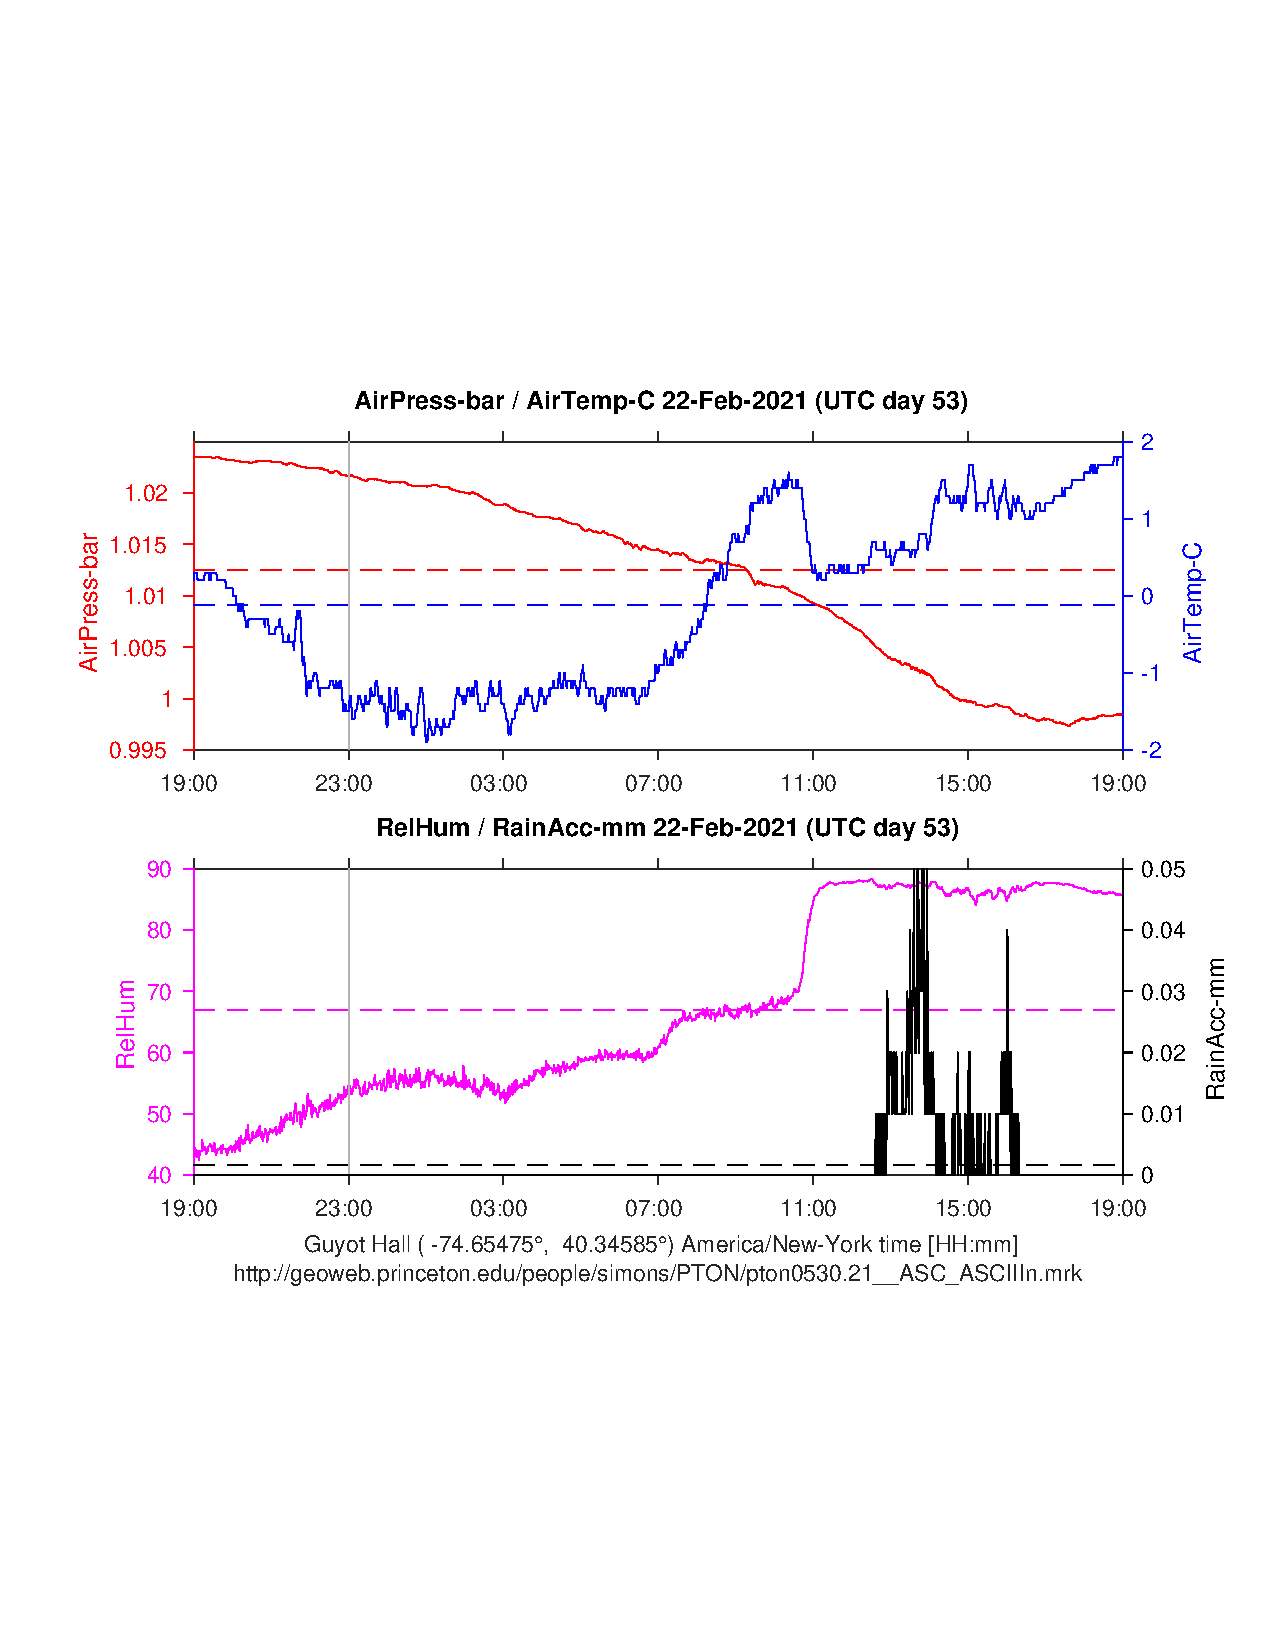
\includegraphics[trim = 0.5cm 5.0cm 0.5cm 6.0cm,clip,width=1.0\textwidth]
{Figures/guyotweather_ywt_feb_22_2021.pdf}
\caption[Weather Station Data]{\label{daily}A daily plot of the
  meteorological variables that the Vaisala station measures on top
  of Guyot Hall.}
\end{figure}

% FJS BASIC CLIMATOLOGY FIGURES TEMPERATURE, PRECIPITATION, RELHUM

From the data analyzed, the following is the climatology of Princeton from
2017 to 2021. Looking at Figure~\ref{Clim1}, we see that we have temperature
and precipitation that varies throughout the year. Temperatures start
increasing before peaking in July, before decreasing until January. This is
consistent with the fact that Princeton has four seasons, which shows cold
winters, warm summers, and mild Spring and Fall. At the same time, there is
more precipitation in the Spring and Summer compared to the relative lack of
precipitation in the Fall and Winter.

The month with the lowest average precipitation is January, at an average
monthly precipitation of 44~mm, whereas the month with the highest average
precipitation is July with 123~mm.

Figure~\ref{Temp_range}, shows that the ranges of temperature are not equal
throughout the months. For example, Winter months of January and Feburary
have a big range that spans from about $20 ^\circ $C to $-10
^\circ$C. Meanwhile, we have Summer months such as July and August, whose
range of temperatures is smaller, from about $30 ^\circ $C to about $15
^\circ $C.

We also see that relative humidity for Princeton is higher in the months of
August to October, whereas the lowest relative humidity seems to be in the
months of March and April.  With Figure~\ref{RH_range}, we can see that all
the months have similar upper extremes of about 90\% for relative humidity,
which can indicate precipitation. At the same time, the range for relative
humidity is largest in the Spring time, with March, April, and May seem to
have a range between 15\% to 90\% for relative humidity, with caution that
this is just data from 3 years.

For atmospheric pressure, the lowest monthly air pressure are found in the
months of April and June, while the highest monthly air pressure are found
in the month of Feburary. Though the values for the mean atmospheric
pressure are all pretty close to each other ranging from about 1.00~bar to
1.01~bar. The more interesting aspects of atmospheric pressure comes from
the range of atmospheric pressure, where the months of May to September all
seem to have a small range that vary between 0.995~bar to about
1.02~bar. Meanwhile we have months like October, which have a larger range
of atmospheric pressure, which ranges from 0.97~bar to 1.03~bar. Clearly
these low atmospheric pressure must come from an intense low pressure that
passed near Princeton and it turns out that for the month of October from
2017-2020, we see that the values between 0.97~bar to 0.985~bar represent
the 0 to 1st percentile of all atmospheric pressures for the month of
October, so they are extremely low pressures. Other months such as November
to February have relatively large ranges for atmospheric pressure as well.
\clearpage
\begin{figure}[b]
	\centering
	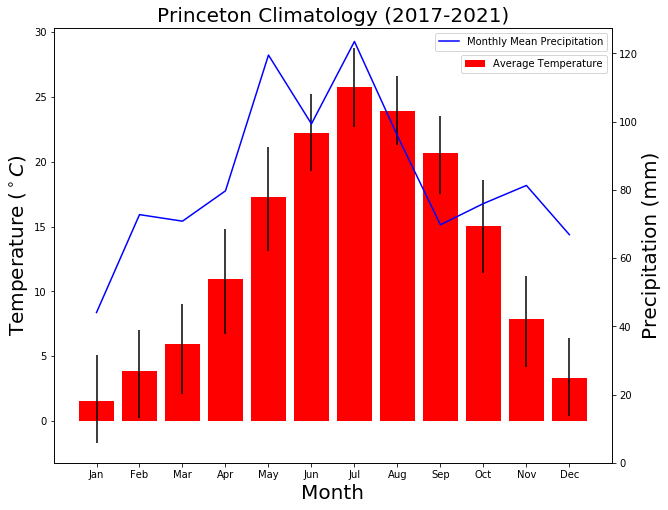
\includegraphics[width=0.675\textwidth]{Figures/Climate1.png}
	\caption[Climatology of temperature and precipitation of Princeton
          (2017--2021)]{\label{Clim1} Climatology shown for Princeton from
          August 2017 to January 2021. The black interval lines show the
          25--75th interpercentile range for temperature of the month.}
\end{figure}

\begin{figure}[b]
	\centering
	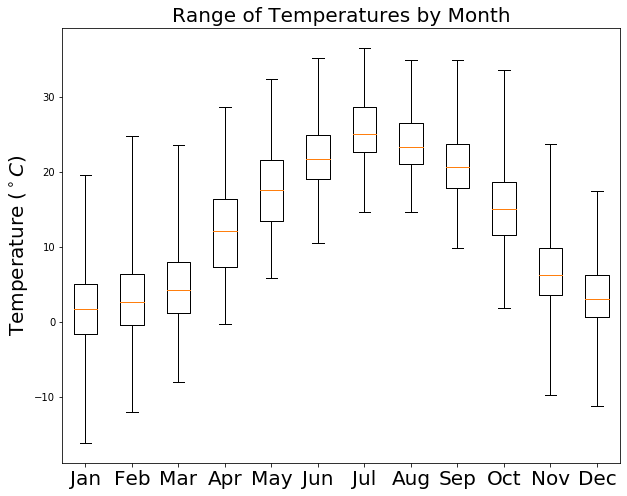
\includegraphics[width=0.675\textwidth]{Figures/Temp_range.png}
	\caption[Temperature range for Princeton
          (2017--2021)]{\label{Temp_range} Shows the interpercentile ranges
          as a bar and the mean temperatures as a line graph. The whiskers
          go out to the 0th percentile and 100th percentile, respectively.}
\end{figure}
\clearpage

%FJS In Section~{\textit{\nameref{sec:dcp}} I show this and that. 
 % Will add 25-75th percentile range, since I think that would make sense. 
  % Again will add 25-75th percentile ranges too, since it would also make sense! 
\clearpage
\begin{figure}[t]
	\centering
	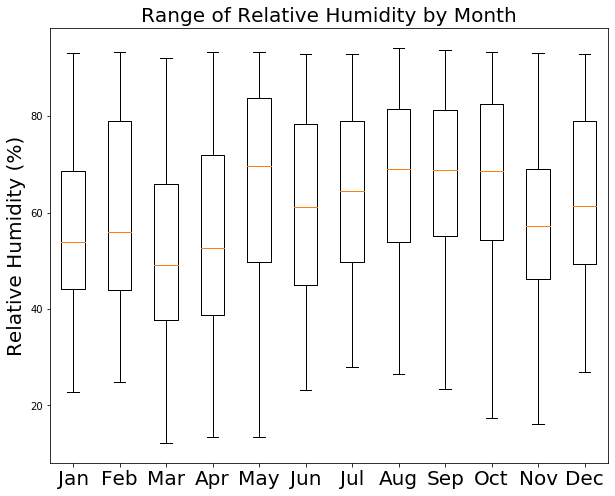
\includegraphics[width=0.65\textwidth]{Figures/RH_range.png}
	\caption[Range of Relative Humidity in Princeton
          (2017--2021)]{\label{RH_range} Range of relative humidity for
          Princeton with the mean relative humidity for the month indicated
          by the orange line.}
\end{figure}
\begin{figure}[b]
	\centering
	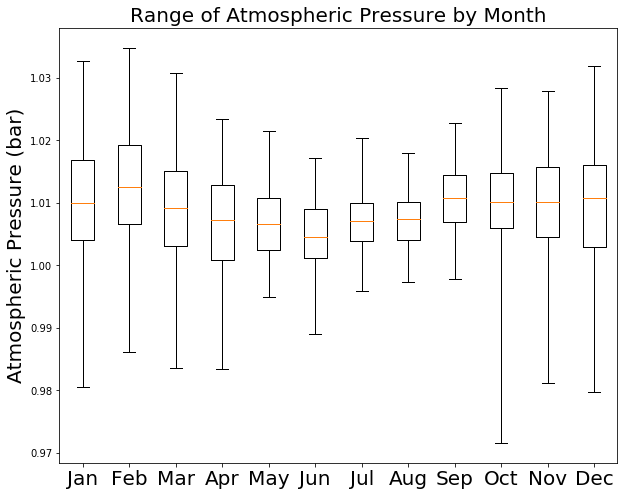
\includegraphics[width=0.65\textwidth]{Figures/AP_range.png}
	\caption[Range of Atmospheric Pressure in Princeton (2017--2021)
        ]{\label{AP_range} A graph similar to Figure~\ref{RH_range} looking
          at range of atmospheric pressure through out the months.}
\end{figure}
\clearpage
\section{Descriptive Climatology of Precipitation}\label{sec:dcp}

Despite the information given to us in looking the ranges of meteorological
variables like temperature, relative humidity, and atmospheric pressure,
precipitation events are no where to be seen.  I shall define the following
terms. The time series of \textbf{precipitation} as recorded by the
instrument is denoted $e_i$, where $i$ indexes the measurement intervals,
each 60~s long. I define a precipitation \textbf{event} $E_j^\tau $ as a
sequence of \textbf{duration} $d_j\ge \tau$ containing contiguous nonzero
precipitation measurements $e_i>0$, flanked left and right by zeros,
$e_i=0$, and where $\tau$ is in minutes \cite[]{Eagleson}.

Furthermore, I define a precipitation \textbf{non-event} $N_j^\tau$, as
having a contiguous set of zeros, $e_i=0$, whose combined duration exceeds
$\tau$, flanked left and right by non-zero values, $e_i=0$ \cite{Eagleson}.
% Basically we want the hand-drawn figure shown here!
One more term to define is \textbf{precipitation intensity}, which for a
precipitation event $E_j^\tau$ is the total amount of precipitation divided
by its duration, i.e.,
\begin{equation}
  I_j^\tau = \fracd{\sum_i e_i }{d_j} ,
  \quad
  \mbox{for}\,\,\,\, i\,\,\,\, \mbox{belonging to the event}\,\,\,\, E_j^\tau
  .
\end{equation}

For further analysis, I am breaking down the year into seasons, as different
seasons may have different characteristics with regards to precipitation. I
will define the seasons as follows: Winter will be December, January, and
February. `Winter' of a certain year contains December of the previous
year. Spring will be March, April, and May. Summer is June, July, and
August. Fall is September, October, November.

These following histograms show the distribution of precipitation event
duration in terms of minutes and shows the different duration distributions
per season. For precipitation and non-precipitation events, $\tau = 1$~min,
which means we will be recording all precipitation events that are 1 minute
or longer in duration. This covers all potential precipitation events.

\clearpage
\begin{figure}[t]
  \centering
  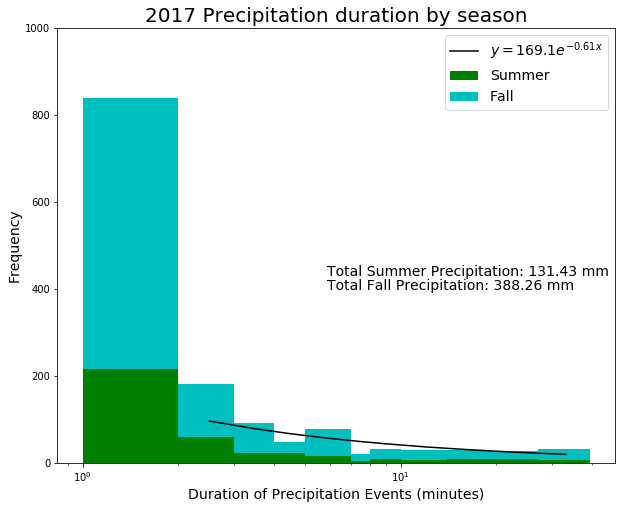
\includegraphics[width=0.675\textwidth]{Figures/precip_2017.png}
  \caption[Precipitation histogram for 2017 broken down by
    season]{\label{p2017} Distribution of precipitation duration in 2017,
    with a breakdown by seasons. The minimum duration is $\tau = 1$~min.
    Note that data collection began on 16 July 2017. Which means we only
    have part of the summer and all of the fall data.  }
\end{figure}
\begin{figure}[b]
  \centering
  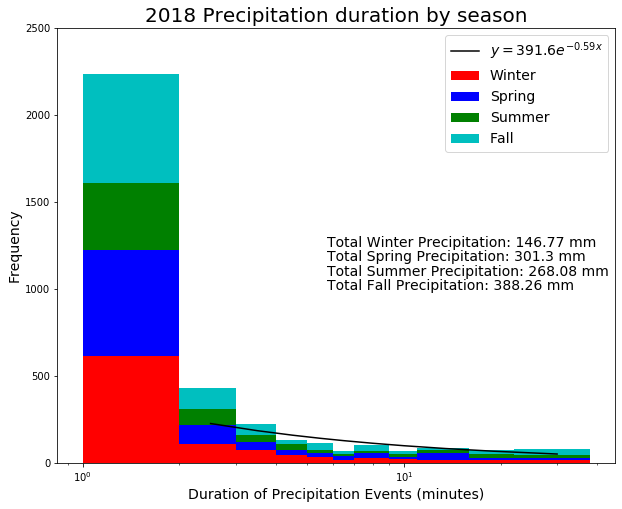
\includegraphics[width=0.675\textwidth]{Figures/precip_2018.png}
  \caption[Precipitation histogram for 2018 broken down by
    season]{\label{p2018} Distribution of precipitation duration in 2018,
    with a breakdown by seasons. 2018 is the first full year of data
    collections. The minimum duration is $\tau = 1$~min.}
\end{figure}

\clearpage
\begin{figure}[t]
 \centering
 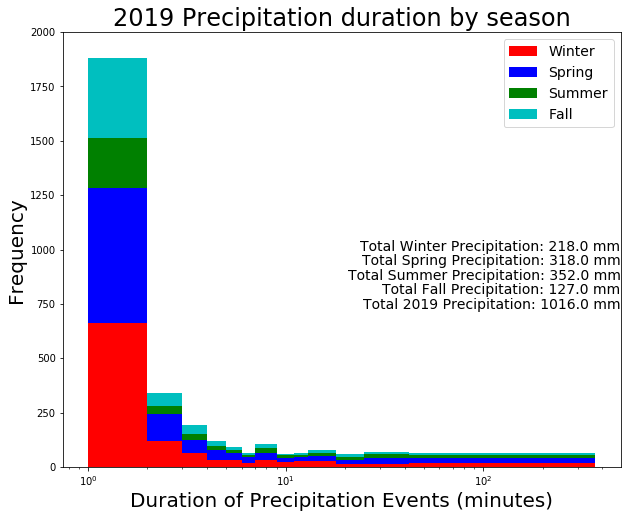
\includegraphics[width=0.675\textwidth]{Figures/precip_2019.png}
 \caption[Precipitation histogram for 2019 broken down by season]
         {\label{p2019}Distribution of precipitation duration in 2019, with
           a breakdown by seasons. The minimum duration is $\tau = 1$~min.
           %The minimum duration, $\tau=1$~min, and the maximum duration over the data
           %set is 368 min, but the horizontal axis was limited to the 98th percentile
           %of the durations, 42~min, for clarity. Superposed is a least-squares fit of
           %a line in log-log space of duration versus frequency for the entire year,
           %excluding the 1--2~min bin, quoted as the equivalent exponential in this
           %space.  
         }
\end{figure}

\begin{figure}[b]
  \centering
  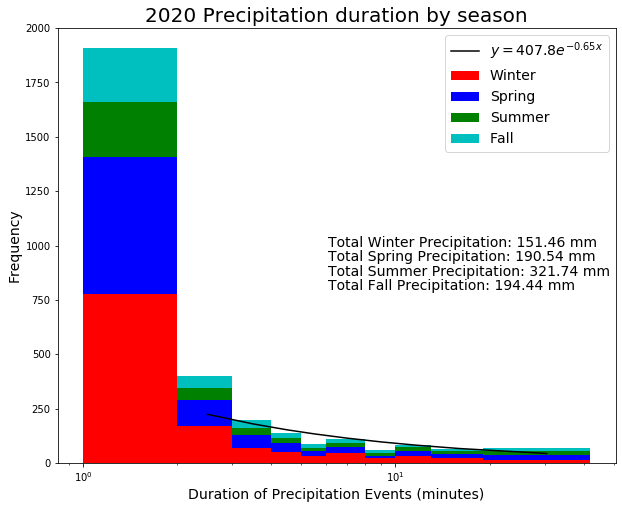
\includegraphics[width=0.675\textwidth]{Figures/precip_2020.png}
  \caption[Precipitation histogram for 2020 broken down by
    season]{\label{p2020} Distribution of precipitation duration in
    2020, with a breakdown by seasons. The minimum duration is $\tau =
    1$~min. %The layout is as in Figure~\ref{p2019}. 
  }
\end{figure}

\clearpage

\begin{figure}[t]
	\centering
	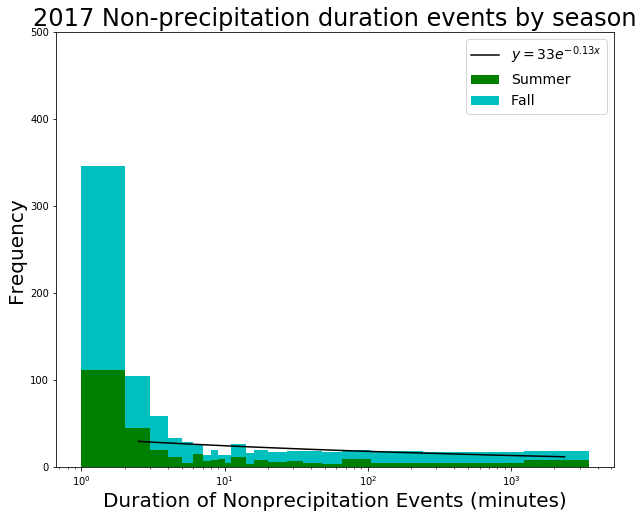
\includegraphics[width=0.675\textwidth]{Figures/nonprecip_2017.png}
	\caption[Histogram of non-precipitation events for 2017 broken down
          by season]{\label{np2017} Distribution of non-precipitation event
          duration in 2017, with a breakdown by seasons. The minimum
          duration is $\tau = 1$~min. Note that data collection began on 16
          July 2017, which means that Summer is only partially complete.}
\end{figure}
\begin{figure}[b]
	\centering
	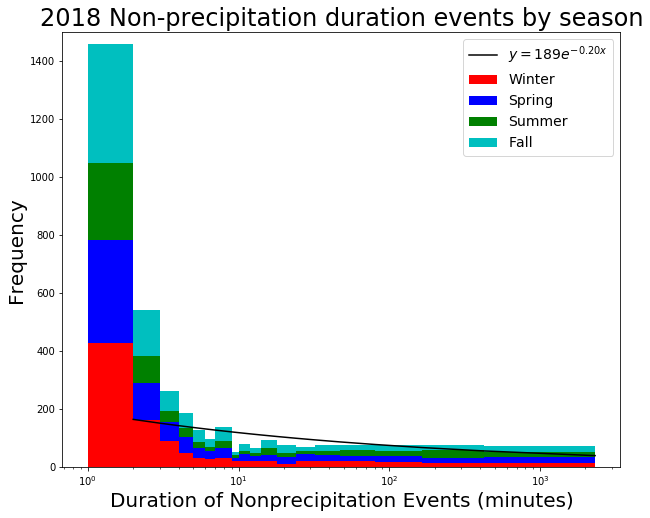
\includegraphics[width=0.675\textwidth]{Figures/nonprecip_2018.png}
	\caption[Histogram of non-precipitation events for 2018 broken down
          by season]{\label{np2018} Distribution of precipitation duration
          in 2018, with a breakdown by seasons. The minimum duration is
          $\tau = 1$~min.}
\end{figure}

\clearpage
\begin{figure}[t]
	\centering
	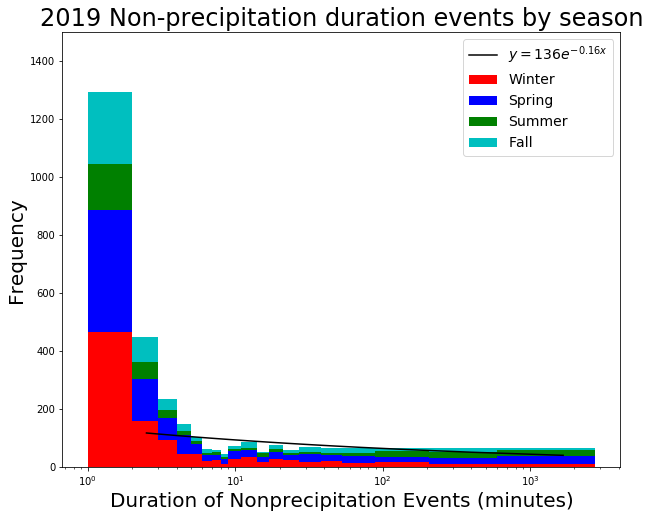
\includegraphics[width=0.675\textwidth]{Figures/nonprecip_2019.png}
	\caption[Histogram of non-precipitation events for 2019 broken
	down by season]{\label{np2019} Distribution of
		non-precipitation event duration in 2019, with a breakdown
		by seasons. The minimum duration is $\tau = 1$~min. %, and the
		%maximum duration over the data set is 2613~min, but the
		%horizontal axis was limited to the 98th percentile of
		%2350~min, for clarity. Superposed is a least-squares fit of
		%a line in log-log space of duration versus frequency for the
		%entire year, excluding the 1--2~min bin, quoted as the
		%equivalent exponential in this space.
	}
\end{figure}

\begin{figure}[b]
	\centering
	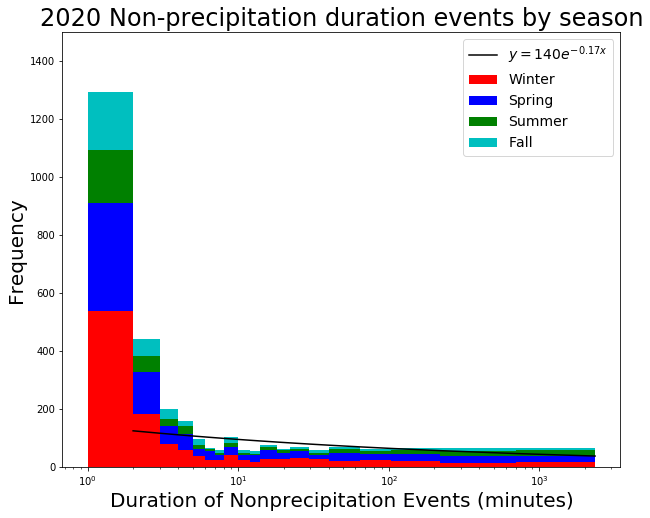
\includegraphics[width=0.675\textwidth]{Figures/nonprecip_2020.png}
	\caption[Histogram of non-precipitation events for 2020 broken down by
	season]{\label{np2020} Distribution of non precipitation event duration
		in 2020, with a breakdown by seasons. The minimum duration is $\tau = 1$~min.}
\end{figure}


\clearpage
\begin{figure}[t]
	\centering
	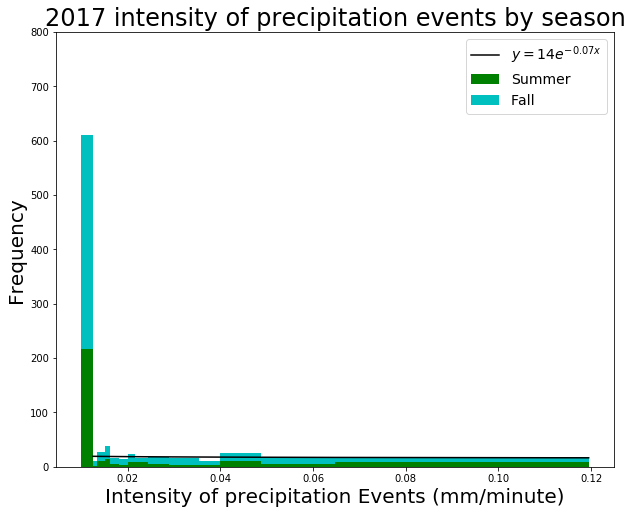
\includegraphics[width=0.675\textwidth]{Figures/inten2017.png}
	\caption[Intensity histogram for 2017 broken down by season]
	{\label{i2017}Distribution of precipitation intensity in 2017,
		with a breakdown by seasons. Note that data collection began on 16
		July 2017. The minimum intensity is
		$I=0.01$~mm/min}
\end{figure}
\begin{figure}[b]
	\centering
	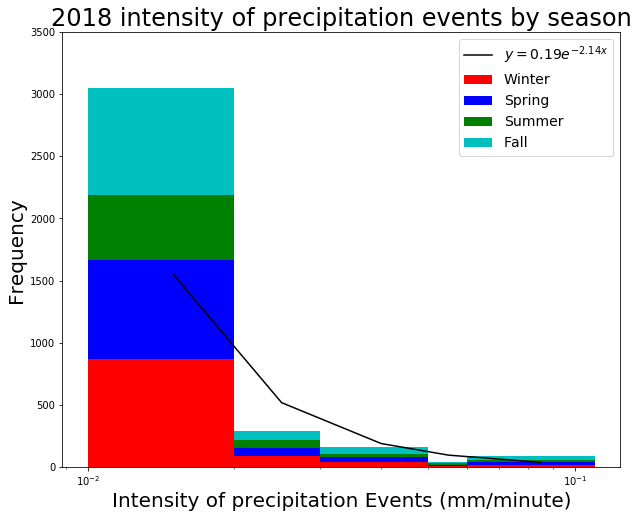
\includegraphics[width=0.675\textwidth]{Figures/inten2018.png}
	\caption[Intensity histogram for 2018 broken down by season]
	{\label{i2018}Distribution of precipitation intensity in 2018,
		with a breakdown by seasons. The minimum intensity is 
		$I=0.01$~mm/min}
\end{figure}
\clearpage
\begin{figure}[t]
	\centering
	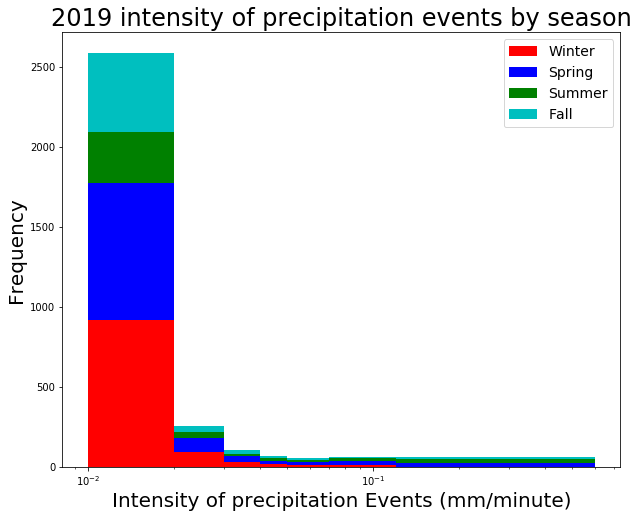
\includegraphics[width=0.675\textwidth]{Figures/inten2019.png}
	\caption[Intensity histogram for 2019 broken down by season]
	{\label{i2019}Distribution of precipitation intensity in
		2019, with a breakdown by seasons. The minimum intensity is
		$I=0.01$~mm/min. 
	}
\end{figure}
\begin{figure}[b]
	\centering
	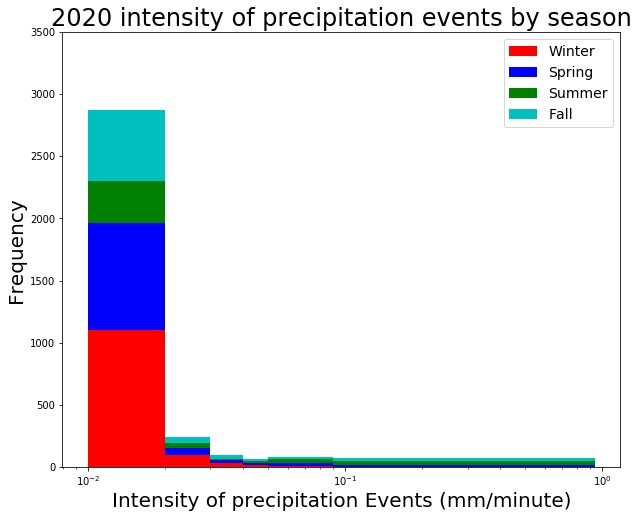
\includegraphics[width=0.675\textwidth]{Figures/inten2020.png}
	\caption[Intensity histogram for 2020 broken down by season]
	{\label{i2020} Distribution of precipitation intensity in
		2020, with a breakdown by seasons. The minimum intensity is
		$I=0.01$~mm/min.}
\end{figure}
\clearpage

These histograms show that the smallest duration events for both
nonprecipitation and precipitation events are the most numerous as seen with
the largest bar in the bins that contain 1 minute to 2 minute durations. The
frequency of duration decreases as we increase the duration bins. At the
same time, there are differences between the precipitation and
non-precipitation events: the upper limit for duration of precipitation
events are about 300 to 400 minutes. However, the upper limit for duration
of non-precipitation events is about an order of magnitude greater at about
2000 minutes. Basically non-precipitation events can be as long as one or
two whole days, where as precipitation events can only last as long as 5-6
hours.

The intensity histogram shows an even stronger aggregation in the lowest
intensity bin of 1~mm/hour to 2~mm/hour. It is interesting because the small
intensity bin can include events that are long but less intense and short,
less intense precipitation events.

\section{Analysis of Precipitation}\label{sec:apc}

% FJS Here I do something. 

\subsection{Methods}\label{sec:methods}

Once we have characterized the climatology of precipitation, we will start
moving towards buidling predictive models for precipitation. In order to see
how accurate such models are in comparison to observed precipitation. Such
accuracy we shall use is to see whether the model and the observed data
match in terms of whether there exists precipitation at a given minute. We
ignore the non-precipitation when looking at accuracy because by matching
non-precipitation minutes in both the model and the observed data, we end up
getting an accuracy of over 90\%, which not useful. So, if the model and the
observed data do not match in terms whether there exists precipitation, this
contributes to the model being deemed less accurate. We can have a stricter
definition of accuracy, in which we set up the precipitation condition, in
addition to saying that the intensity must match too, otherwise we can not
say the model and observed data match. This stricter definition of model
accuracy might be used when thinking about

\subsection{Results}\label{sec:apcr}

Figure~\ref{p2019} shows the distribution of durations of 3198 precipitation
events $E_j^1$, i.e. $E_j^\tau$ where $\tau=1$~min for the year 2019, broken
down by season. In order to make bins that contain non-zero values, I
created bins using duration percentiles. I used unique values obtained from
using a range of percentiles from 0 to 100, in 2 and 5 percent
intervals. For one analysis, I stopped at 98 \% believing this would be the
best approach in terms of fitting. At the same time, I also made sure to
analyze the data including the 100 percentile, to see how it differs when
including the extremes. Such purpose is also to realize that excluding such
extremes produced modelled precipitation that did not last long as well as
well as the gaps between precipitation events being too small.

I used an exponential fit to the frequency-duration histograms for all 1253
events $E_j^2$, i.e. $E_j^\tau$ where $\tau=2$~min. For all the other years,
as shown in Figures~\ref{p2020}, \ref{p2018} and~\ref{p2017}, I used a
similar procedure. Excluding the first interval shown, focusing on events of duration
greater than or equal to 2~min, we propose an exponential model for
the histogram, with the following equation:
\begin{equation}\label{expod}
  F = \beta \,e^{\alpha d},
\end{equation}
where $F$ is the frequency and $d$ the duration, and with $\beta$ the
unitless frequency coefficient and $\alpha$ is the exponential coefficient
(in units of min$^{-1}$). Table~\ref{firsttable} shows the
coefficients~$\beta$ and the exponential coefficients~$\alpha$ from looking
at the yearly frequency of precipitation duration.

We shall also propose the following equations which will also describe an
exponential model for the histogram regarding non-precipitation events,
which is described by the following equation:
\begin{equation}\label{expod_np}
	F_{np} = \gamma \,e^{\delta D},
\end{equation}
where $F_{np}$ is the frequency of non-precipitation events, $D$ being
duration, and $\gamma $ being the unitless frequency coefficient and $\delta
$ is the exponential coefficient. Table~\ref{thirdtable_98} shows the
coefficients~$\gamma$ and exponential coefficients~$\delta$ from looking at
yearly frequency of non-precipitation event durations.

A similar equation for precipitation intensity can be described by the
following equation:
\begin{equation}\label{expod_inten}
	F_{inten} = \epsilon \,e^{\zeta I},
\end{equation}
where $F_{inten}$ is the frequency of intensity of precipitation events, $I$
is the intensity of the precipitation events, $\epsilon$ is the unitless
frequency coefficient, and $\zeta$ is the exponential
coefficient. Table~\ref{fourthtable} shows the coefficients~$\epsilon$ and
the exponential coefficients~$\zeta$ from looking at yearly frequency of
intensity of precipitation events.

\clearpage
\begin{figure}[t]
\centering
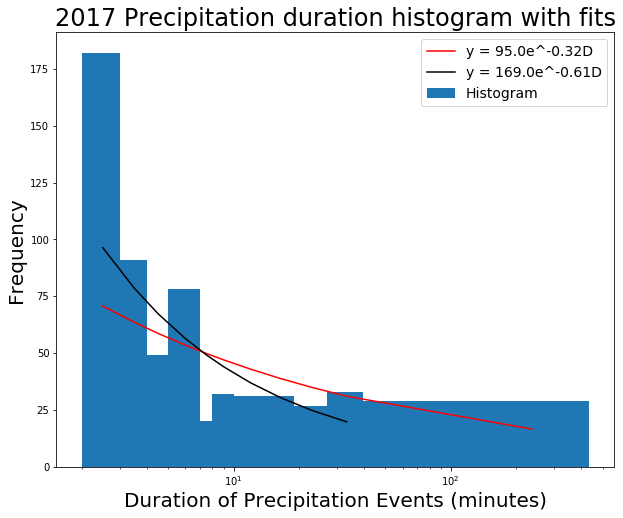
\includegraphics[width=0.625\textwidth]{Figures/precip17_new.png}
\caption[2017 precipitation duration exponentials with contrasting curve fitting]
{\label{precip17_redone}Curve fitting of the precipitation histogram
  excluding 1 minute duration events for the incomplete 2017 data. The red
  curve denotes the curve that fits to the 100th percentile, while the black
  curve fits the data to the 98th percentile. Has similar trends to the
  other years, though 2017 has incomplete data.}
\end{figure}

\begin{figure}[b]
\centering
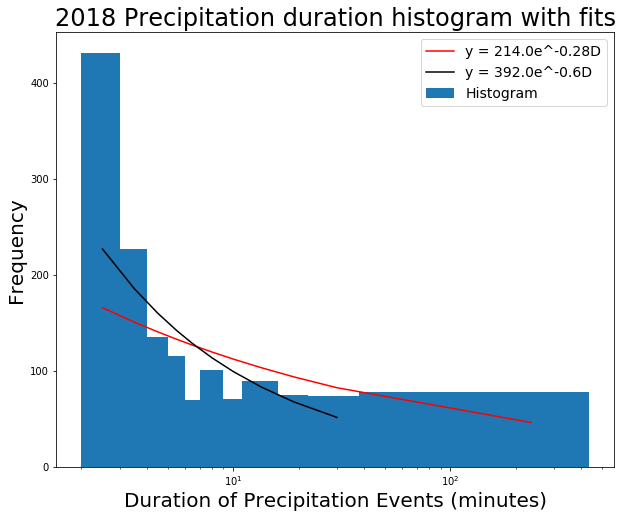
\includegraphics[width=0.625\textwidth]{Figures/precip18_new.png}
\caption[2018 precipitation duration exponentials with contrasting curve fitting]
{\label{precip18_redone}Curve fitting of the precipitation histogram
  excluding 1 minute duration events for the entire 2018 data. Format is the
  same as Figure~\ref{precip17_redone}, with the understanding that 2018 has
  complete data.}
\end{figure}

\clearpage

\begin{figure}[t]
\centering
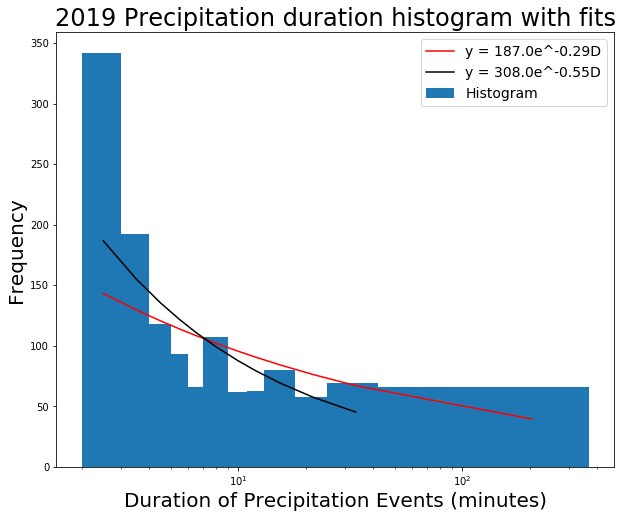
\includegraphics[width=0.675\textwidth]{Figures/precip19_new.png}
\caption[2019 precipitation duration exponentials with contrasting curve fitting]
{\label{precip19_redone}Curve fitting of the precipitation histogram
  excluding 1 minute duration events for the entire 2019 data. The layout is
  the same as seen in Figure~\ref{precip17_redone}, with 2019 having complete data
  like 2018. 2018 and 2019 have similar trends and similar curves for both
  best fit curves.}
\end{figure}

\begin{figure}[b]
\centering
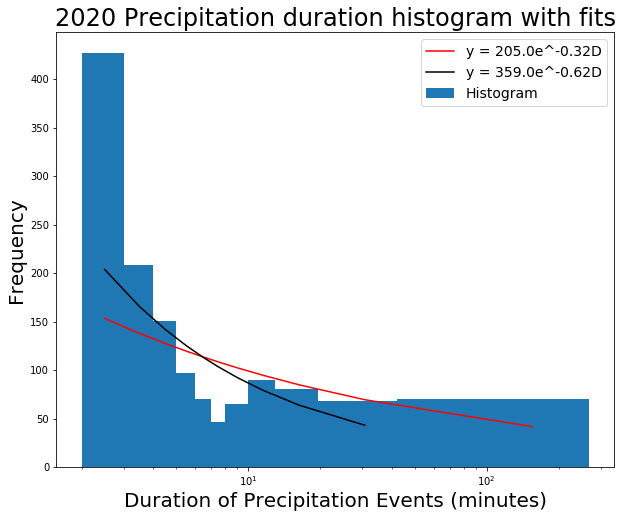
\includegraphics[width=0.675\textwidth]{Figures/precip20_new.png}
\caption[2020 precipitation duration exponentials with contrasting curve fitting]
{\label{precip20_redone}Curve fitting of the histogram excluding 1
  minute duration events for the entire 2020 data. The layout is the same as
  seen in Fig\ref{precip17_redone} with 2020 having completed data as
  well. 2018, 2019, and 2020 all look similar looking at the histogram and
  the best fit curves.}
\end{figure}

\clearpage
\begin{figure}[t]
\centering
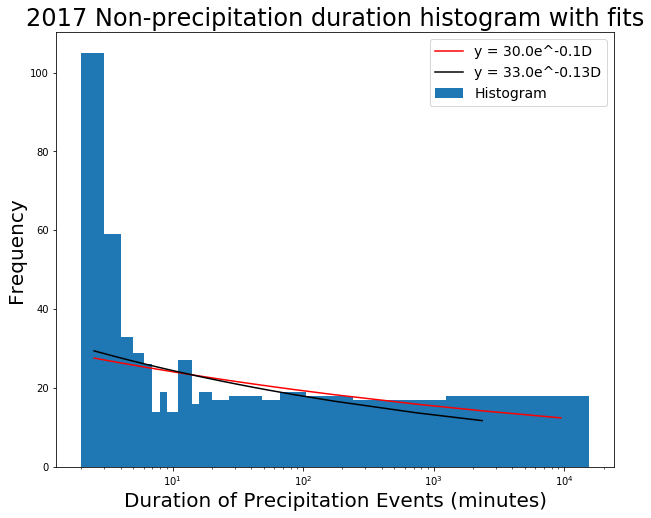
\includegraphics[width=0.625\textwidth]{Figures/nonprecip_2017_new.png}
\caption[2017 Non-precipitation duration Exponentials with contrasting curve fitting]

{\label{nonprecip17_redone}Curve fitting of the histogram excluding 1 minute
  duration events for the incomplete 2017 data. The red curve denotes the
  curve that fits to the 100th percentile, while the black curve fits the
  data to the 98th percentile. Has similar trends to the other years, though
  2017 has incomplete data.}
\end{figure}

\begin{figure}[b]
  \centering
  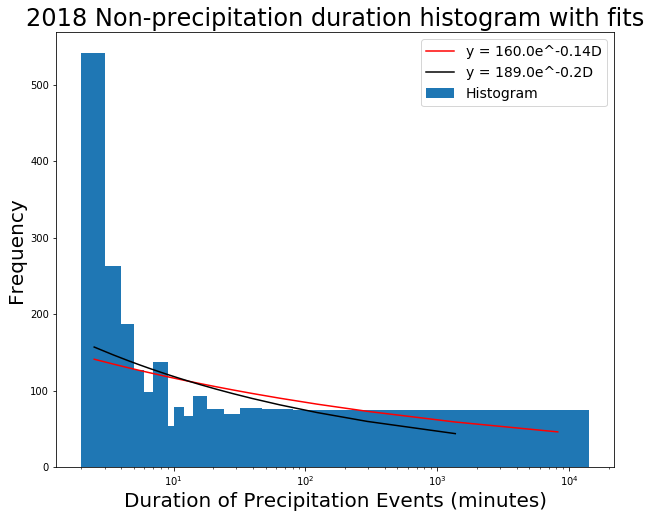
\includegraphics[width=0.625\textwidth]{Figures/nonprecip_2018_new.png}
  \caption[2018 Non-precipitation duration Exponentials with contrasting curve fitting]
  {\label{nonprecip18_redone} Shows curve fitting of the histogram excluding
    1 minute duration events for the entire 2018 data. The red curve denotes
    the curve that fits to the 100th percentile, while the black curve fits
    the data to the 98th percentile. The 98 percentile curve fitting the
    smaller durations better, while the 100 percentile curve fitting the
    larger durations better.  Perhaps the only real difference between 2017
    and 2018 is the frequency, with 2018 having complete data.}
\end{figure}

\clearpage

\begin{figure}[t]
  \centering
  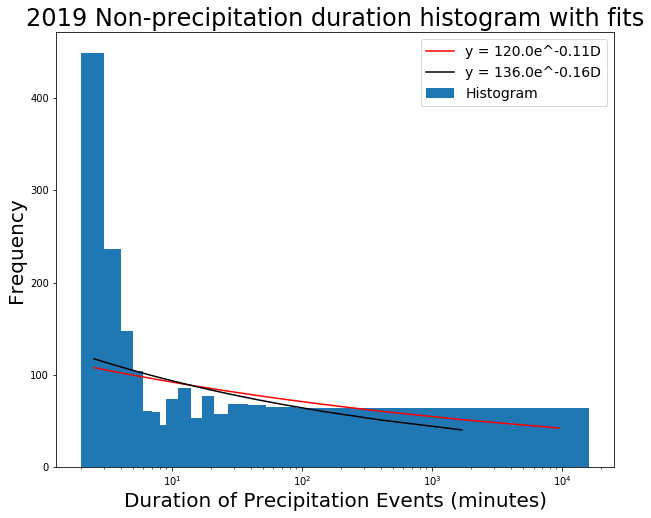
\includegraphics[width=0.675\textwidth]{Figures/nonprecip_2019_new.png}
  \caption[2019 Non-precipitation duration Exponentials with contrasting curve fitting]
  {\label{nonprecip19_redone} Shows curve fitting of the histogram excluding
    1 minute duration events for the entire 2019 data. The layout is the
    same as seen in Figure~\ref{precip18_redone}. 2018 and 2019 have similar trends
    and similar curves for both best fit curves.}
\end{figure}

\begin{figure}[b]
  \centering
  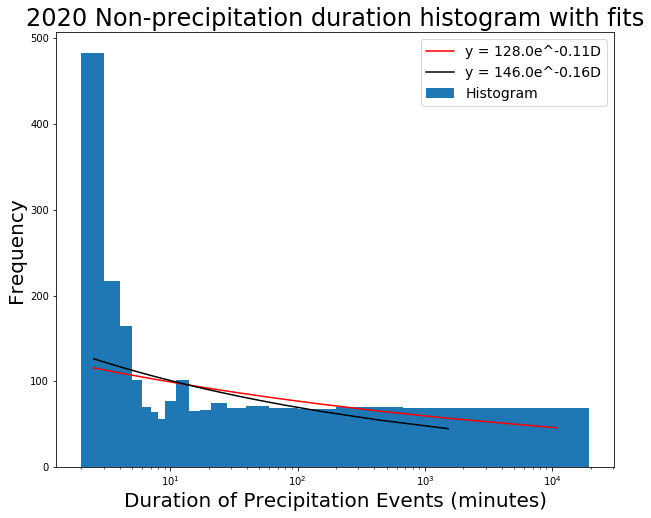
\includegraphics[width=0.675\textwidth]{Figures/nonprecip_2020_new.png}
  \caption[2020 Non-precipitation duration Exponentials with contrasting curve fitting]
  {\label{nonprecip20_redone}Curve fitting of the histogram excluding
    1 minute duration events for the entire 2020 data. The layout is the
    same as seen in Figure~\ref{nonprecip18_redone}. 2018, 2019, and 2020 all look
    similar looking at the histogram and the best fit curves.}
\end{figure}

%Is the exponential different for W/S/S/F? Can you tell the difference?
%Is the exponential different for different years? Can you tell the
%difference?  And what summarizes it all. 
\clearpage
\begin{figure}[t]
  \centering
  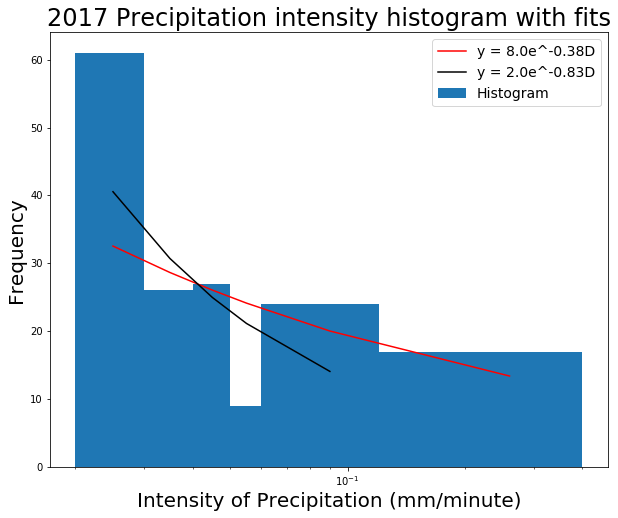
\includegraphics[width=0.675\textwidth]{Figures/inten2017_fit.png}
  \caption[Fitting Intensity histogram for 2017 with different bins]
          {\label{i2017_fit} Curve fitting of the histogram excluding the
            1~mm/minute intensity bin for the 2017 data that was
            collected. The black curve fits up to the 98th percentile
            bin. The red curve fits up to the 100th percentile bin. The
            black curve fits the lower bins better, but the red curve fits
            to include the extremes better.  }
\end{figure}

\begin{figure}[b]
  \centering
  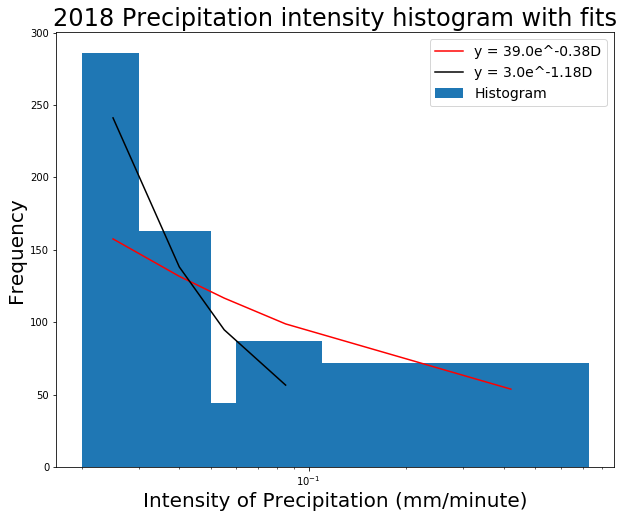
\includegraphics[width=0.675\textwidth]{Figures/inten2018_fit.png}
  \caption[Fitting Intensity histogram for 2018 with different bins]
          {\label{i2018_fit} Curve fitting of the histogram excluding the 1
            mm/minute intensity bin for the entire 2018 data. The layout is
            the same as Figure~\ref{i2017_fit}, with the red curve fitting
            the extremes better, while the black curve fits the lower
            intensity bins better.}
\end{figure}

\clearpage
\begin{figure}[t]
  \centering
  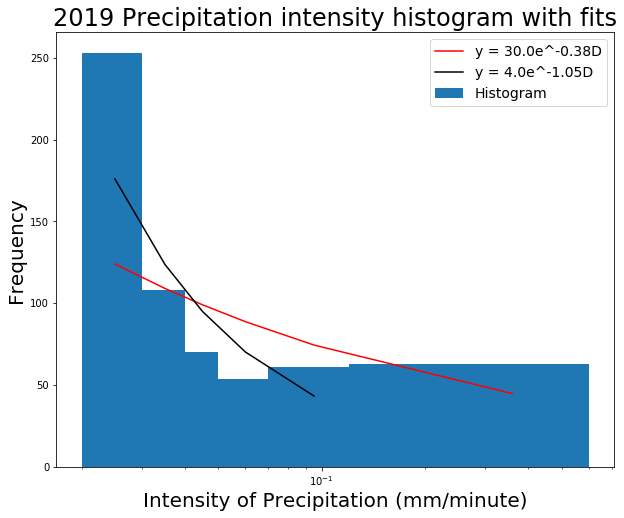
\includegraphics[width=0.675\textwidth]{Figures/inten2019_fit.png}
  \caption[Fitting Intensity histogram for 2019 with different bins]
          {\label{i2019_fit} Curve fitting of the histogram excluding the 1
            mm/minute intensity bin for the entire 2019 data. The layout is
            the same as Figure~\ref{i2017_fit}, with the red curve fitting
            the extremes better, while the black curve fits the lower
            intensity bins better.  }
\end{figure}

\begin{figure}[b]
  \centering
  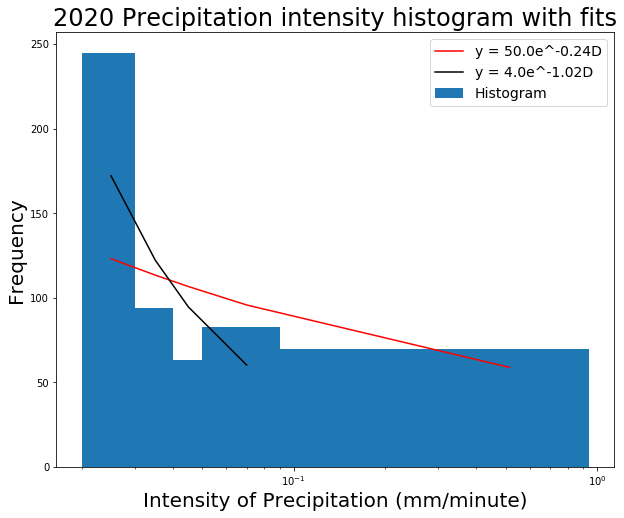
\includegraphics[width=0.675\textwidth]{Figures/inten2020_fit.png}
  \caption[Fitting Intensity histogram for 2020 with different bins]
          {\label{i2020_fit} Curve fitting of the histogram excluding the 1
            mm/minute intensity bin for the entire 2020 data. The layout is
            the same as Figure~\ref{i2017_fit}, with the red curve fitting
            the extremes better, while the black curve fits the lower
            intensity bins better.  }
\end{figure}

\clearpage

\subsection{Discussion}\label{sec:apcd}


Table~\ref{firsttable} show that $\beta$ values are similar to each other
with the exception of 2017, which only had partial data starting in the
Summer. Even with the partial data that we have from 2017 and 2020, it is
clear that the $\alpha$ values are similar to each other. Focusing on the
years with complete data, 2018 and 2019, it is clear that yearly variations
exist between them. All $\alpha$ values are negative.\\[-1.5em]

\begin{table}[bh]
  \begin{center}
    \begin{tabular}{|l|*{11}{r|}r|}
      \hline
      Season    &       \multicolumn{2}{|c|}{Annual}          & \multicolumn{2}{|c|}{Winter}& \multicolumn{2}{|c|}{Spring}  & \multicolumn{2}{|c|}{Summer} &\multicolumn{2}{|c|}{Fall}  \\
      \hline
      Year      & $\beta $ & $\alpha$  & $\beta $ & $\alpha$ & $\beta $ & $\alpha$ & $\beta $ & $\alpha$ & $\beta $ & $\alpha$\\
      \hline
      2017      & \textit{169}  & \textit{-0.61}  & NaN & NaN & NaN & NaN & \textit{57}  & \textit{-0.70}  & 108  & -0.57  \\
      2018      & 392           & -0.59  & 148 & -0.74 & 125 & -0.76 & 65  & -0.52  & 91 & -0.50  \\
      2019      & 308           & -0.54  & 118  & -0.62 & 107 & -0.58 & 32 & -0.31  & 57 &  -0.60 \\
      2020      & 408           & -0.65   & 201  & -0.80 & 112  & -0.66 & 48  & -0.42 & 64 & -0.66\\
      \hline
    \end{tabular}
  \end{center}
\caption[Year comparison of coefficients of precipitation duration up to its
  98th percentile]{\label{firsttable}Coefficients found from the yearly
  distribution of precipitation duration (as in equation~\ref{expod}) as
  well as the seasonal distribution of precipitation duration. Italics refer
  to values obtained using incomplete information. NaN means there was no
  information. These coefficients were computed using the 0 to 98th
  percentile of precipitation duration.}
\end{table}


\begin{table}[htb]
  \begin{center}
    \begin{tabular}{|l|*{11}{r|}r|}
      \hline
      Season    &       \multicolumn{2}{|c|}{Annual}          & \multicolumn{2}{|c|}{Winter}& \multicolumn{2}{|c|}{Spring}  & \multicolumn{2}{|c|}{Summer} &\multicolumn{2}{|c|}{Fall}  \\
      \hline
      Year      & $\beta $ & $\alpha$  & $\beta $ & $\alpha$ & $\beta $ & $\alpha$ & $\beta $ & $\alpha$ & $\beta $ & $\alpha$\\
      \hline
      2017      & \textit{94}  & \textit{-0.32}  & NaN & NaN & NaN & NaN & \textit{32}  & \textit{-0.14}  & 68  & -0.09  \\
      2018      & 214           & -0.28  & 73 & -0.37 & 46 & -0.27 & 38  & -0.24  & 55 & -0.23  \\
      2019      & 224          & -0.28  & 68  & -0.34 & 60 & -0.28 & 25 & -0.19  & 33 &  -0.32 \\
      2020      & 234           & -0.35   & 119  & -0.51 & 60  & -0.32 & 36  & -0.27 & \textit{29} & \textit{-0.23}\\
      \hline
    \end{tabular}
  \end{center}
\caption[Yearly comparison of
  coefficients of precipitation duration using 0 to 100th percentile]{\label{firsttable_100} Coefficients found from the yearly
  distribution of precipitation duration (as in equation~\ref{expod})
  as well as the seasonal distribution of precipitation
  duration. Italics refer to values obtained using incomplete
  information. NaN means there was no information. These coefficients were computed using the all the data, from 0 to 100th percentile.}
\end{table}


In the seasonal variations, we see that Summer has $\alpha$ values that are
less negative compared to the other seasons as well as having a lower
$\beta$ compared to the other seasons.  The Spring appears to mimic the
Winter in that there are a lot of preciptiation events, but also shares the
quality of Summer in having fairly high precipitation totals. The Fall
shares the Summer quality of having relatively few preciptation events, but
tends to have smaller precipitation totals, so its intensity is less than
the Summer, but greater than the winter precipitation intensity.

Compared to Table~\ref{firsttable}, Table~\ref{firsttable_100} seems to show
$\beta$ values that are consistently lower when considering the 100th
percentile bins for precipitation event durations. The $\alpha$ values are
also less negative, which better reflects that there are extreme durations
for precipitation events.

\ 

\begin{table}[htb]
  \begin{center}
    \begin{tabular}{|l|*{11}{c|}r|}
      \hline Season & \multicolumn{2}{|c|}{Annual} &
      \multicolumn{2}{|c|}{Winter}& \multicolumn{2}{|c|}{Spring} &
      \multicolumn{2}{|c|}{Summer} &\multicolumn{2}{|c|}{Fall} \\ \hline
      Year & $\gamma $ & $\delta$ & $\gamma $ & $\delta$ & $\gamma $ &
      $\delta$ & $\gamma $ & $\delta$ & $\gamma $ & $\delta$\\ \hline 2017 &
      \textit{33} & \textit{-0.13} & NaN & NaN & NaN & NaN & \textit{12} &
      \textit{-0.15} & 19 & -0.12 \\ 2018 & 189 & -0.20 & 59 & -0.28 & 50 &
      -0.29 & 26 & -0.10 & 55 & -0.22 \\ 2019 & 136 & -0.16 & 63 & -0.30 &
      46 & -0.16 & 11 & 0.03 & 24 & -0.16 \\ 2020 & 140 & -0.17 & 64 & -0.23
      & 46 & -0.16 & 13 & -0.02 & 20 & -0.21 \\ \hline
    \end{tabular}
  \end{center}
  \caption[Year comparison of coefficients for non-precipitation events up
    to 98th percentile] {\label{thirdtable_98}Coefficients found from
    the yearly distribution of non-precipitation event duration (as in
    equation~\ref{expod_np}) as well as the seasonal distribution of
    non-precipitation event duration. Italics refer to values obtained using
    incomplete information. NaN means there was no information. Using
    non-precipitation event durations from the 0 to the 98th percentile.}
\end{table}


\begin{table}[htb]
  \begin{center}
    \begin{tabular}{|l|*{11}{c|}r|}
      \hline
      Season    &       \multicolumn{2}{|c|}{Annual}          & \multicolumn{2}{|c|}{Winter}& \multicolumn{2}{|c|}{Spring}  & \multicolumn{2}{|c|}{Summer} &\multicolumn{2}{|c|}{Fall}  \\
      \hline
      Year      & $\gamma $ & $\delta$  & $\gamma $ & $\delta$ & $\gamma $ & $\delta$ & $\gamma $ & $\delta$ & $\gamma $ & $\delta$\\
      \hline
      2017      & \textit{30}  & \textit{-0.10}  & NaN & NaN & NaN & NaN & \textit{11}  & \textit{-0.10}  & 18  & -0.09  \\
      2018      & 160           & -0.14  & 47 & -0.19 & 43 & -0.14 & 23  & -0.05  & 46 & -0.15  \\
      2019      & 120           & -0.11  & 49 & -0.21 & 44 & -0.15 & 11 & 0.04 & 19 & -0.08   \\
      2020      & 121           & -0.11  & 57 & -0.19 & 41 & -0.12 & 12  & 0.01  & 15 & -0.11 \\
      \hline
    \end{tabular}
  \end{center}
  \caption[Year comparison of coefficients for non-precipitation events up
    to 100th percentile] {\label{thirdtable_100}Coefficients found from the
    yearly distribution of non-precipitation event duration (as in
    equation~\ref{expod_np}) as well as the seasonal distribution of
    non-precipitation event duration. Italics refer to values obtained using
    incomplete information. NaN means there was no information. Using
    non-precipitation event durations from the 0 to 100th percentile.}
\end{table}


When fitting non-precipitation event durations using the exponential model,
the coefficients $\delta$ are less negative overall compared to the
coefficients of the precipitation event duration, $\alpha$.

Some of this difference is explained by the fact that the durations of
non-precipitation events range from 1 minute to over 2000 minutes, whereas
the durations of precipitation events range from 1 minute to just over
300--400 minutes. Also, how we bin the durations for both precipitation and
non-precipitation events will affect how we get the fits.

Once again, taking into the account the most extreme durations for
non-precipitation events lowers the frequency value of $\gamma$ and the
exponential constant of $\delta$ is less negative, when comparing
Table~\ref{thirdtable_98} and Table~\ref{thirdtable_100}.

\

\begin{table}[htb]
  \begin{center}
    \begin{tabular}{|l|*{11}{c|}r|}
      \hline
      Season    &       \multicolumn{2}{|c|}{Annual}          & \multicolumn{2}{|c|}{Winter}& \multicolumn{2}{|c|}{Spring}  & \multicolumn{2}{|c|}{Summer} &\multicolumn{2}{|c|}{Fall}  \\
      \hline
      Year      & $\epsilon $ & $\zeta$  &  $\epsilon $ & $\zeta$  &  $\epsilon $ & $\zeta$  &  $\epsilon $ & $\zeta$  & $\epsilon $ & $\zeta$ \\
      \hline
      2017      & \textit{0.06}  & \textit{-1.98}  & NaN & NaN & NaN & NaN & \textit{0.03}  & \textit{-1.94}  & 0.04  & -2.00  \\
      2018      & 0.19           & -2.14  & 0.02 & -2.41 & 0.03 & -2.24  & 0.10  & -1.87  & 0.08 & -2.05  \\
      2019      & 0.23           & -2.01  & 0.03 & -2.29 & 0.07 & -2.02 & 0.25 & -1.47 & 0.03 & -2.16  \\
      2020      & 0.06          & -2.38  & 0.002 & -3.00 & 0.02 & -2.38 & 0.10  & -1.74 & 0.02 & -2.18\\
      \hline
    \end{tabular}
  \end{center}
  \caption[Year comparison of coefficients for precipitation
    intensity] {\label{fourthtable}Coefficients found from the yearly
    distribution of precipitation intensity (as in equation~\ref{expod_inten}) as
    well as the seasonal distribution of precipitation
    intensity. Italics refer to values obtained using incomplete
    information. NaN means there was no information. }
\end{table}


\begin{table}[htb]
  \begin{center}
    \begin{tabular}{|l|*{11}{c|}r|}
      \hline
      Season    &       \multicolumn{2}{|c|}{Annual}          & \multicolumn{2}{|c|}{Winter}& \multicolumn{2}{|c|}{Spring}  & \multicolumn{2}{|c|}{Summer} &\multicolumn{2}{|c|}{Fall}  \\
      \hline
      Year      & $\epsilon $ & $\zeta$  &  $\epsilon $ & $\zeta$  &  $\epsilon $ & $\zeta$  &  $\epsilon $ & $\zeta$  & $\epsilon $ & $\zeta$ \\
      \hline
      2017      & \textit{1.6}  & \textit{-1.05}  & NaN & NaN & NaN & NaN & \textit{0.8}  & \textit{-0.94}  & 0.8  & -1.12 \\
      2018      & 12           & -0.919  & 0.7 & -1.36 & 3 & -0.91  & 6  & -0.67  & 4 & -0.91  \\
      2019      & 9           & -0.94  & 0.10 & -1.9 & 3 & -0.94 & 7 & -0.48 & 1 & -1.0  \\
      2020      & 16          & -0.76  & 0.5 & -1.4 & 3 & -0.86 & 13  & -0.32 & 3 & -0.69\\
      \hline
    \end{tabular}
  \end{center}
  \caption[Year comparison of coefficients for precipitation
    intensity using 0 to 100 percentile] {\label{fourthtable_100}Coefficients found from the yearly
    distribution of precipitation intensity (as in equation~\ref{expod_inten}) as
    well as the seasonal distribution of precipitation
    intensity. Italics refer to values obtained using incomplete
    information. NaN means there was no information. Using intensity from 0 to 100th percentile. }
\end{table}


In contrast, Table~\ref{fourthtable} for intensity of precipitation events
show a more negative exponential compared to either precipitation or
non-precipitation event durations. This is partially due to the fact that
there are fewer bins in the intensity of preciptiation events as seen that
the vast majority of precipitation events are not particularly intense on
average.

The differences between Table~\ref{fourthtable} and
Table~\ref{fourthtable_100} show that the exponential coefficients for
intensity clearly are changed most when the 98th percentile or the 100th
percentile are included in the fit. First, the $\epsilon$ value increases
when we use the 100th percentile rather than the 98th
percentile. Furthermore, we see that the $\zeta$ value also becomes less
negative, but very dramatically compared to non-precipitation and
precipitation event durations.

However, Table~\ref{secondtable} shows that the Summers also have a lot of
precipitation. There may be fewer precipitation events, but their total
precipitation is higher, hence they have a higher intensity.  For the
Winter, the $\alpha$ are the furthest from 0 and the $\beta$ are
large. However, Winters tend to have the lowest values for total
precipitation and the combination of lots of preciptation events and low
precipitation totals results in the lowest intensities among the four
seasons.

\begin{table}[t]
  \begin{center}
    \begin{tabular}{|l|*{11}{c|}r|}
      \hline
      Season    &       \multicolumn{2}{|c|}{Annual}          & \multicolumn{2}{|c|}{Winter}& \multicolumn{2}{|c|}{Spring}  & \multicolumn{2}{|c|}{Summer} &\multicolumn{2}{|c|}{Fall}  \\
      \hline
      Year      & T & I  & T & I  & T & I  & T & I  & T & I \\
      \hline
      2017      & \textit{520}  & \textit{0.07}  & NaN & NaN & NaN & NaN & \textit{131}  & \textit{0.07}  & 388  & 0.07  \\
      2018      & 1104           & 0.06  & 147 & 0.03 & 301 & 0.07 & 268  & 0.08  & 388 & 0.07  \\
      2019      & 1016           & 0.06  & 218  & 0.04 & 318 & 0.06 & 352 & 0.11  & 127 &  0.05 \\
      2020      & 858          & 0.06   & 151  & 0.03 & 191  & 0.04 & 322  & 0.12 & 194 & 0.06\\
      \hline
    \end{tabular}
  \end{center}
  \caption[Summary of total precipitation and
    intensity]{\label{secondtable}Total precipitation (in mm) and average
    intensity (in mm/min) of precipitation for each year and season. Italics
    refer to values obtained using incomplete information. NaN means there
    was no information.}
\end{table}

\clearpage

\section{Simulation for Prediction}\label{sec:sfp}

\subsection{Method}\label{sec:sfp_m}

To make a base line model, we need to first use the exponentials that we
calculated for the duration of the precipitation event, intensity of the
precipitation event, and duration of the non-precipitation events. However,
we also need to manually add back in the lowest durations and lowest
intensities, since we excluded those values when calculating the exponential
distributions. To perform the simulation, we select bins proportionally to
their probability under the distributino, and then pick values from a
uniform distribution with those bins.

\clearpage 

\subsection{Results}\label{sec:sfp_r}

\begin{figure}[t]
  \centering
  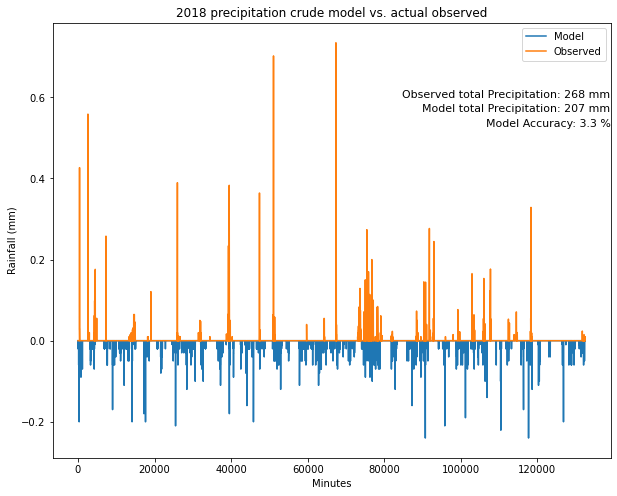
\includegraphics[width=0.75\textwidth]{Figures/better_one_run.png}
  \caption[One run using Summer 2018 climatology] {\label{crudemodel}One
    model run using the exponentials calculated from Summer 2018.}
\end{figure}

Running the model one hundred times let us look at what the average
precipitation total the model yields, it yields 195 mm compared to the
Summer 2018 total of 268 mm that we used. Furthermore, the accuracy of model
precipitation matching model precipitation is only 6$\%$. Looking at
\ref{crudemodel}, we see that the model precipitation total is lower than
the actual precipitation observed in the Summer of 2018. Furthermore, the
precipitation seem to be more frequent compared to the observed 2018 Summer
data.

It is clear that despite the better fit using the curve fit of 98th
percentile, we need to use the 100th percentile, since the extremes such as
the big 2000 minute non-precipitation even is very important in the nature
of the precipitation event. However, it is clear that the accuracy does not
improve significantly. The fact that the model total precipitation is still
less than from the initial observed precipitation shows how this model needs
more improvement.
\clearpage

\begin{figure}[t]
  \centering
  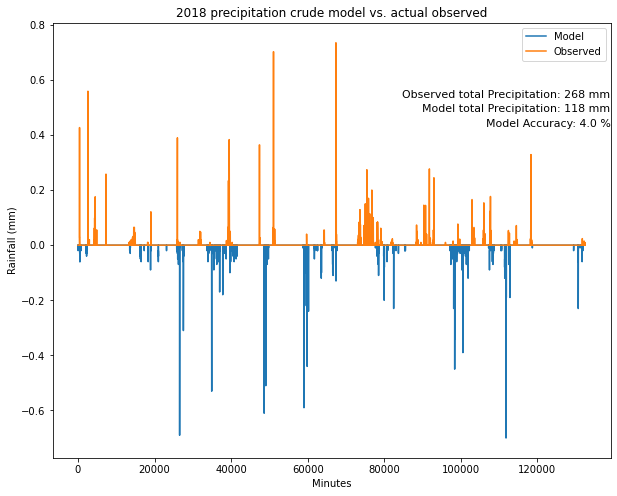
\includegraphics[width=0.75\textwidth]{Figures/best_one_run.png}
  \caption[Modified run using Summer 2018 climatology]
  {\label{crudermodel} One model run using the exponentials calculated from
    Summer 2018. Made some adjustments to get a better match for the actual
    summer 2018 run.}
\end{figure}

\begin{figure}[b]
  \centering
  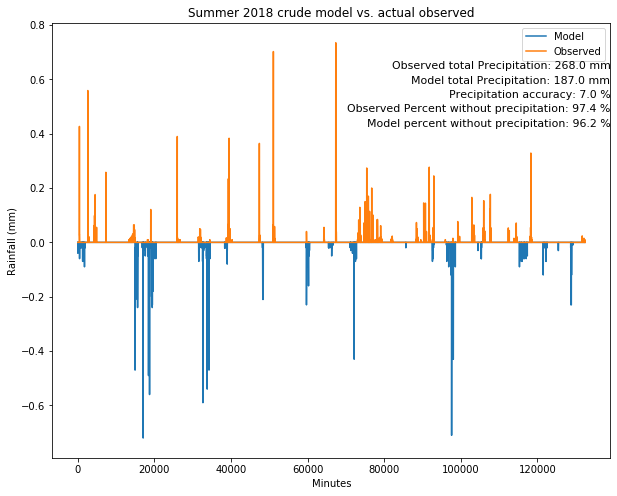
\includegraphics[width=0.75\textwidth]{Figures/run_with_more_info.png}
  \caption[More  run using Summer 2018 climatology]
  {\label{crudesmodel} One model run using the exponentials calculated from
    Summer 2018. Put up some more information such as how much of the time
    was non-dominated by no precipitation.}
\end{figure}
\clearpage

\subsection{Discussion}\label{sec:spc_d}


\section{Machine Learning for Prediction}\label{sec:MLP}

% FJS Simulation from learned exponential fits gives you a baseline

% FJS ML approach random forest gives you new results

% FJS Contrast with a traditional multiple linear regression

% FJS take into account the time frame for lagged prediction

\subsection{Method}

We can see that despite the flaws that we get from the exponential fits,
this gives us a good baseline to start off.

\subsection{Results}

\subsection{Discussion}


\clearpage

\section{Discussion and Conclusions}\label{sec:conclusions}

%--References
\small
\renewcommand{\bibsep}{0em}

\renewcommand{\bibname}{References}
\bibliographystyle{Latex/gji}
\bibliography{refs}

\end{document}
